% Informe de Proyecto % Autor: Tu Nombre % Fecha: Fecha actual

\documentclass[11pt,a4paper]{article}

\usepackage[spanish]{babel} 
\usepackage[utf8]{inputenc} 
\usepackage{graphicx}
\usepackage{hyperref}

\title{Actas Capitulares de la Habana} \author{Edian Broche Castro \\ Roger Fuentes Rodr\'iguez \\ Kevin Manzano Rodr\'iguez \\ Massiel Paz Otaño \\ Jackson Claudio Vera Pineda} \date{}

\begin{document}

\maketitle

\tableofcontents

\section{Introducción}
\subsection{Objetivo del Proyecto} 

Se tiene como objetivo desarrollar una propuesta de transcripción y procesamiento de un conjunto de imagenes, para su posterior uso como dataset en futuros proyectos para identificar entidades nombradas y crear grafos de conocimiento.  

\subsection{Contexto}

Se tiene una serie documental perteneciente al fondo Ayuntamiento de La Habana del Archivo Histórico de la Oficina del Historiador de la Ciudad de la Habana.

Esta serie documental se divide en dos grupos o subseries: los libros originales (1550 - 1898) y los libros trasuntados (1550 - 1809). Los primeros destacan por su riqueza de contenido y forma; los segundos por dejar constancia de la labor del Ayuntamiento para garantizar la perdurabilidad en el tiempo de este tipo documental, al ser copias realizadas en la segunda mitad del siglo XIX.

Las actas dejan la huella de una institución colonial y su devenir en el tiempo: el Ayuntamiento. Ellas recogen los planteamientos y discusiones de aquellos problemas que interesaron a los pobladores del lugar, ya fueran de índole económica, política o social; están reflejados los hechos mas significativos de cada una de las épocas.

Se tiene como corpus el tomo 1 digitalizado, el resto está en proceso de digitalización.

\section{Metodología} 
\subsection{Enfoque del Proyecto} 

Existen m\'ultiples herramientas para la transcripción de documentos hist\'oricos entre estas destacan \href{https://www.transkribus.org/}{Transkribus} la cual fue recomendada por el cliente por su uso en anteriores trabajos, pero debido al deterioro de los documentos adem\'as del tipo espec\'ifico de tipograf\'ia los resultados no eran satisfactorios. Debido al bajo \textbf{accuracy} provisto por esta herramienta creada por especialistas en el tema podemos asumir que el problema es bastante complejo.

\begin{center} 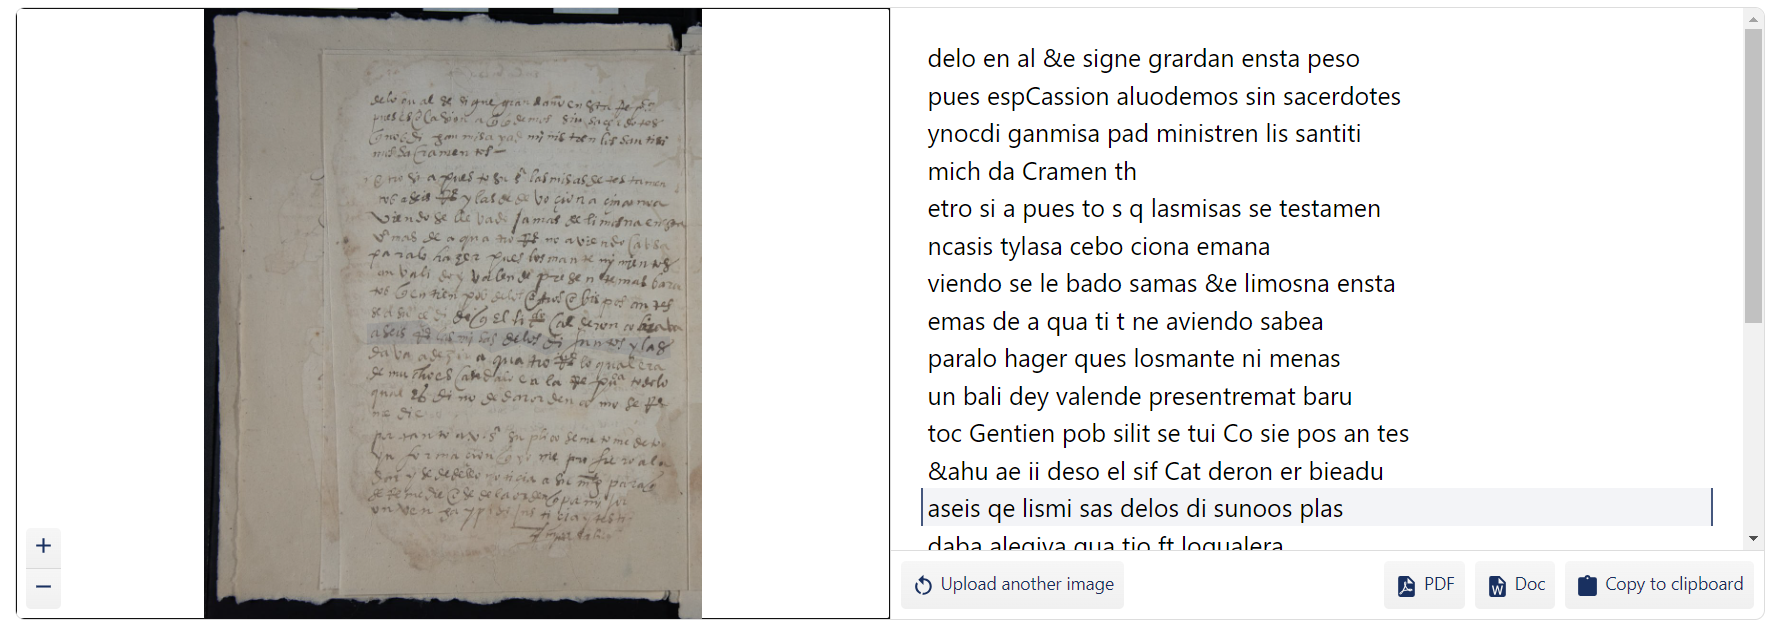
\includegraphics[width=1.0\textwidth]{transkribus} \end{center}

Nos encontramos con dos grandes problemas, falta de datos para llevar a cabo un entrenamiento de alg\'un modelo pues muchos de los datasets encontrados no poseen el idioma requerido (Español) ni el tipo de letra (procesal-cortesana), y una tarea que solo un ojo humano especializado podr\'ia realizar (tip\'ografo)

Debido a todo lo expuesto el proyecto fue enfocado en una b\'usqueda exhaustiva de datos clasificados, un procesamiento minucioso de las im\'agenes, el uso de varios OCRs, y un posprocesamiento con diccionarios del idioma y LLM.

\subsection{Recursos Utilizados}

Como lenguaje principal se utilizo python, debido a que brinda un f\'acil acceso a librerias de procesamiento de texto e im\'agenes. Entre las librerias utilizadas destacan \textbf{Kraken}, \textbf{PIL}, \textbf{TensorFlow}, \textbf{Numpy},  \textbf{matplotlib}, \textbf{scipy}, \textbf{spacy}, \textbf{symspellpy} y \textbf{transformers}.

El LLM utilizado fue \textbf{Gemini} por cuestiones económicas, como diccionario de frequencias utilizamos \href{https://github.com/hermitdave/FrequencyWords/blob/master/content/2016/es/es_full.txt}{spanish frequency dictionary} (se considero la creaci\'on de un diccionario a partir de un libro escrito por Luis XV pero se tendr\'ian muy pocas palabras en comparaci\'on con el utilizado), el modelo de spacy utilizado fue \textbf{es core news sm}.

Entre los datos recopilados inicialmente se utiliz\'o \href{https://zenodo.org/records/1490009/files/Rodrigo%20corpus%201.0.0.tar.gz?download=1}{dataset de rodrigo} es un dataset de Español antiguo, pero la tipograf\'ia no coincide, en este caso se utiliza letra g\'otica, luego se encontr\'o todo un corpus de documentos en Español de años anteriores a 1900 \href{https://corpuscodea.es/}{CODEA} y con una estructura que podiamos aprovechar, la mayor\'ia de los documentos presentan una triple representaci\'on, la imagen, una transcripción paleogr\'afica, y una presentanci\'on cr\'itica. El dataset inicialmente tiene alrededor de 4000 documentos, pero luego de filtrar por el tipo de letra requerida se reduce a 546, recalcando la dificultad de los datos.

AQUI FALTAN AGREGAR COSAS

\section{Resultados} 
\subsection{Logros Principales} 

En la primera etapa del producto se logra una mejora considerable en la imagen, se utiliza un pipeline para limpiar las im\'agenes con t\'ecnicas de filtrado como filtro Gaussiano para reducir el ruido general de la imagen y un filtro de mediana para reducir el ruido sal y pimienta. Se emplea un algoritmo de detecci\'on de bordes Canny para identificar letras presentes en los documentos, pero esto solamente deja los bordes por lo que se aplican luego operaciones morfol\'ogicas de dilataci\'on y erosi\'on para reconstruir el trazo. Se intento el uso de algoritmos como sobel y laplaciano , el \'ultimo no funciono bien porque depende de la segunda derivada de los cambios pixel a pixel, y esto en documentos de texto donde el documento es blanco y las letras son negras y los cambios de papel tinta son muy abruptos indefine la derivada y causo malos resultados. Adem\'as se probo binarizaci\'on de la imagen, definiendo un umbral de intensidad donde si $x >$ threshold se toma como letra y en caso contrario como fondo , pero en zonas de sombra , probando con diferentes valores para threshold no se detecta bien la escritura, tambi\'en se intento binarizaci\'on adaptativa pero se recuperaba mucho ruido y manchas en el documento. Para el tratado de las manchas debido a la longevidad de los documentos(son amarillos) se implement\'o un conversor personalizado de la imagen de color a escala de grises ponderando las componentes rgb de forma diferente a lo usual (que es el promedio), r + g es el equivalente al amarillo por lo que se pondero r y g en menor grado jugando con los par\'ametros para tratar de contrarestar el ruido.

\begin{figure}[h] \centering \begin{minipage}{1.0\textwidth} 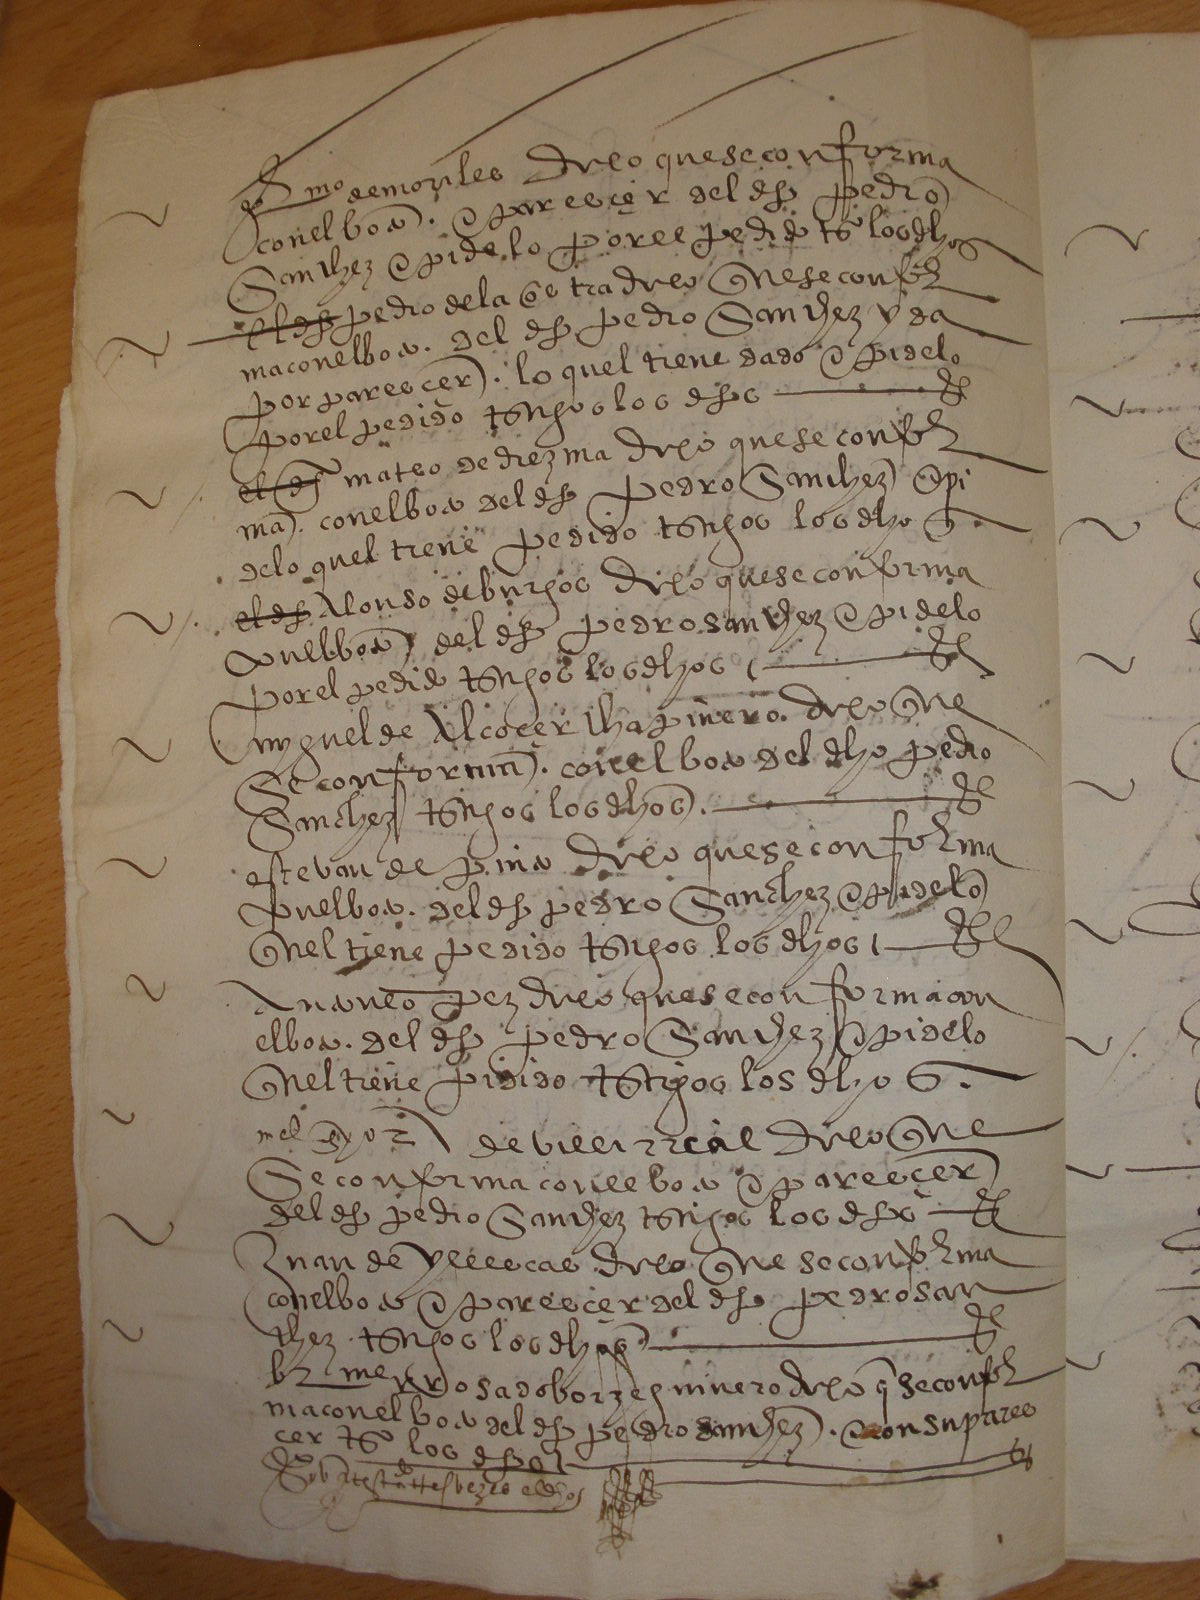
\includegraphics[width=0.32\textwidth]{CODEA-0205_2v.jpg} 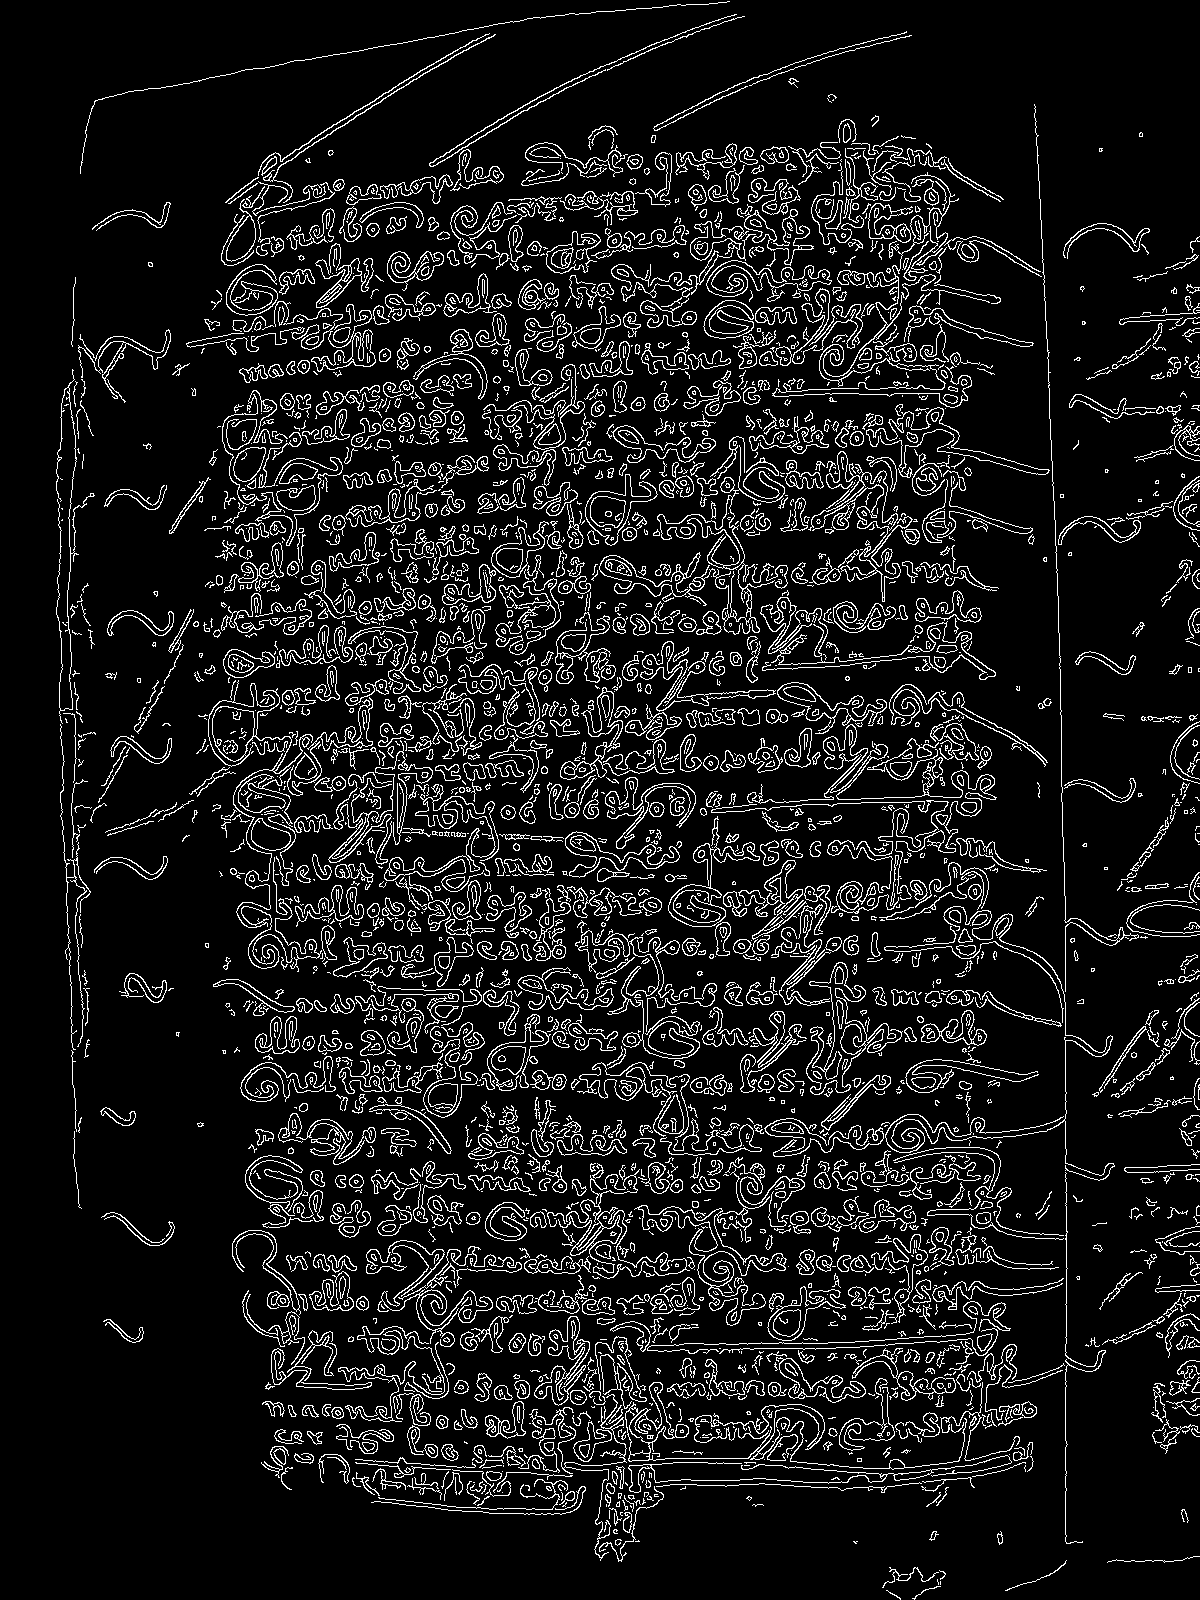
\includegraphics[width=0.32\textwidth]{canny_image_aftergauss_eq2.png} 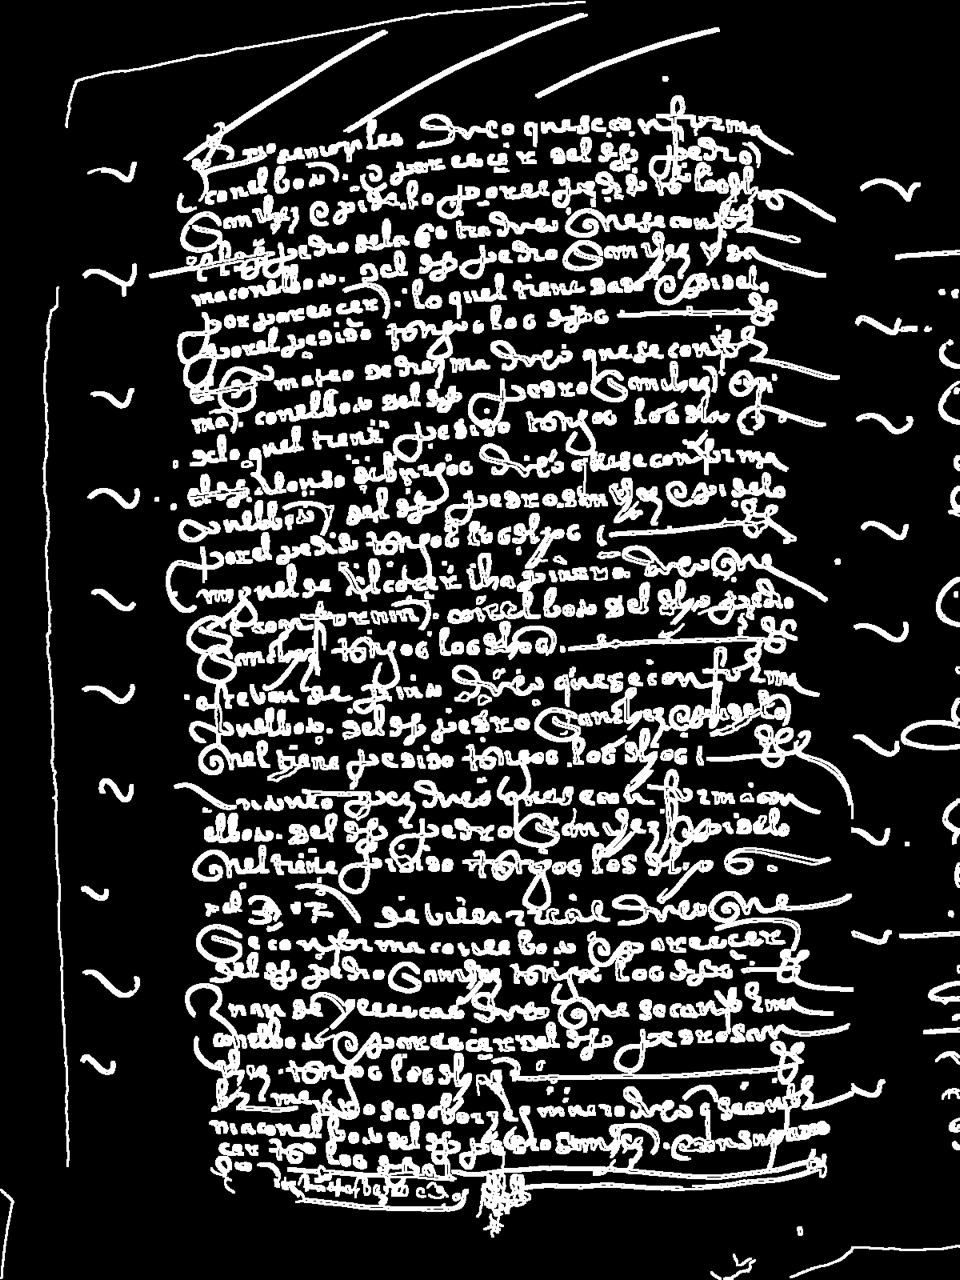
\includegraphics[width=0.32\textwidth]{photo_2025-01-27_21-34-01.jpg} \caption{Original, detecci\'on de bordes, operaciones morfol\'ogicas de izquieda a derecha} \label{fig:tresfotos} \end{minipage} \end{figure}
Luego de binarizadas las im\'agenes son pasadas por dos procesos de segmentación, uno que brinda \textbf{Kraken} y una proyecci\'on de histogramas, se sugiere utilizar la primera pues otorga mejores resultados, y en caso de un proceso manual ser\'ia mejor utilizar \textbf{SAM2} pero no logramos automatizar el proceso, luego de segmentada la imagen esta es pasada a 3 OCRs distintos, \textbf{SimpleHTR}, \textbf{sinai-sam-rec-v4-best}, \textbf{McCATMuS-nfd-nofix-V1}, los cuales son modelos especializados en \textbf{handrwitten recognition}, los dos \'ultimos provienen de Kraken, aqu\'i tuvimos que tratarlos diferentes pues, el primero necesita la imagen segmentadas y los otros solamente los \textbf{bounding box}.

En la \'ultima etapa una vez procesadas la im\'agenes con las t\'ecnicas para mejorarlas y luego extraido el texto con los diferentes OCRs, se realiz\'o un posprocesamiento para mejorar la calidad de las transcripciones, inspirados en el DataSet de CODEA, brindamos una transcripción cr\'itica del documento. Dada la naturaleza de los documentos y los errores inherentes al OCR, implementamos un pipeline para corregir errores ortogr\'aficos y ajustar la chorencia del texto, de esta forma refinando la salida.

Se utiliz\'o un modelo de lenguaje \textbf{Spacy} para segmentar el texto en tokens, para as\'i identificar palabras y elementos no alfab\'eticos. Cada token fue corregido utilizando SymSpell, una herramienta basada en un diccionario de frecuencias, para separar correctamente palabras unidas y capitalizarlas. Tras  las correcciones se utiliz\'o un modelo generativo, Gemini para realizar un refinamiento sem\'antico y estil\'istico; corrigiendo as\'i el formato del texto y la gram\'atica, adem\'as de mantener el contexto hist\'orico del español antiguio. Tambi\'en se consideraron las diferentes salidas y se combinaron en una sola.

A continuaci\'on un ejemplo del flujo:

\begin{enumerate}
    \item Essta es una prueva de ectraccion de teexto. Connoscida cosa sea a todos los queesta carta uieren como yo don Fferrando por la gracia de dios hey de Castiella
    \item Esta es una prueba de extracción de texto. Conocida cosa sea a todos los que esta carta vieren como yo don Fferrando por la gracia de Dios hay de Castilla
    \item Esta es una prueba de extracción de texto. Conocida cosa sea a todos aquellos que esta carta vieran, como yo, don Fernando, por la gracia de Dios, rey de Castilla.
\end{enumerate}

\subsection{Desafíos Superados}

En el momento de la segmentación jug\'o un papel fundamental la b\'usqueda de par\'ametros adecuados para que tuviera mejor rendimiento los procesos posteriores.

Entre los desaf\'ios superados en el posprocesamiento nos encontramos con la conservaci\'on del español antiguo pues no encontramos un diccionario de frecuencias de esa época, pero solventamos este problema con el LLM utilizado, la obtención del mismo fue compleja, pues se probaron con otros, por ejemplo \textbf{GPT-2}, \textbf{"google/mt5-small"}, \textbf{flax-community/spanish-t5-small}, pero los resultados fueron p\'esimos en los tres casos, adem\'as de que no ten\'iamos un API c\'omoda y los modelos eran bastantes pesados, por lo que optamos por \textbf{Gemini}.

\section{Conclusiones} \subsection{Impacto del Proyecto} \subsection{Recomendaciones para Futuras Implementaciones}

\appendix \section{Anexos} \subsection{Documentación Adicional} \subsection{Códigos Fuente}

\bibliographystyle{plain} \bibliography{referencias}

\end{document} $